%%%%%%%%%%%%%%%%%%%%%%%%%%%%%%%%%%%%%%%%%%%%%%%%%%%%%%%%%%%%%%%%%%%%%%%%%%%%%%%%%%
\begin{frame}[fragile]\frametitle{}

\begin{center}
{\Large Word Embeddings in Gensim}

{\tiny (Ref: How to Develop Word Embeddings in Python with Gensim - Jason Brownlee)}
\end{center}

\end{frame}

%%%%%%%%%%%%%%%%%%%%%%%%%%%%%%%%%%%%%%%%%%%%%%%%%%%%%%%%%%%%%%%%%%%%%%%%%%%%%%%%%%
\begin{frame}[fragile]\frametitle{Word Embeding (recap)}

\begin{itemize}
\item A word embedding is an approach to provide a dense vector representation of words that capture something about their meaning.

\item Word embeddings are an improvement over simpler bag-of-word model word encoding schemes like word counts and frequencies that result in large and sparse vectors (mostly 0 values) that describe documents but not the meaning of the words.

\item Word embeddings work by using an algorithm to train a set of fixed-length dense and continuous-valued vectors based on a large corpus of text. Each word is represented by a point in the embedding space and these points are learned and moved around based on the words that surround the target word.
\end{itemize}
\end{frame}


%%%%%%%%%%%%%%%%%%%%%%%%%%%%%%%%%%%%%%%%%%%%%%%%%%%%%%%%%%%%%%%%%%%%%%%%%%%%%%%%%%
\begin{frame}[fragile]\frametitle{Word2Vec }

Learning a word embedding from text involves loading and organizing the text into sentences and providing them to the constructor of a new Word2Vec() instance. For example:
\begin{lstlisting}
sentences = [['..','..','....'],[],[],...]
model = Word2Vec(sentences)
\end{lstlisting}
Specifically, each sentence must be tokenized, meaning divided into words and prepared 
\end{frame}


%%%%%%%%%%%%%%%%%%%%%%%%%%%%%%%%%%%%%%%%%%%%%%%%%%%%%%%%%%%%%%%%%%%%%%%%%%%%%%%%%%
\begin{frame}[fragile]\frametitle{Preparing the Input}
gensim's word2vec expects a sequence of sentences as its input. Each sentence a list of words (utf8 strings): 
\begin{lstlisting}
sentences = [['first', 'sentence'], ['second', 'sentence']]
# train word2vec on the two sentences
model = gensim.models.Word2Vec(sentences, min_count=1)
\end{lstlisting}
\begin{itemize}
\item Keeping the input as a Python built-in list is convenient, but can use up a lot of RAM when the input is large. 
\item Gensim only requires that the input must provide sentences sequentially, when iterated over. 
\item No need to keep everything in RAM: we can provide one sentence, process it, forget it, load another sentence
\end{itemize}
\end{frame}

%%%%%%%%%%%%%%%%%%%%%%%%%%%%%%%%%%%%%%%%%%%%%%%%%%%%%%%%%%%%%%%%%%%%%%%%%%%%%%%%%%
\begin{frame}[fragile]\frametitle{Preparing the Input}
\begin{lstlisting}
model = gensim.models.Word2Vec(iter=1)  # an empty model, no training yet
model.build_vocab(some_sentences)  # can be a non-repeatable, 1-pass generator
model.train(other_sentences)  # can be a non-repeatable, 1-pass generator
\end{lstlisting}
\begin{itemize}
\item Calling Word2Vec(sentences, iter=1) will run two passes over the sentences iterator (or, in general iter+1 passes; default iter=5). 
\item The first pass collects words and their frequencies to build an internal dictionary tree structure. 
\item The second and subsequent passes train the neural model. 
\item You can store/load models using the standard gensim methods: 
\end{itemize}
% \begin{lstlisting}
% model.save('/tmp/mymodel')
% new_model = gensim.models.Word2Vec.load('/tmp/mymodel')
% \end{lstlisting}
\end{frame}



% %%%%%%%%%%%%%%%%%%%%%%%%%%%%%%%%%%%%%%%%%%%%%%%%%%%%%%%%%%%%%%%%%%%%%%%%%%%%%%%%%%
% \begin{frame}[fragile]\frametitle{Training your own word vectors}
% Word2Vec requires that every document is contained in a list and every list contains list of tokens of that documents. 

% \begin{lstlisting}
% docs=[['Neeraj','Boy'],['Sarwan','is'],['good','boy']] 
% #training word2vec on 3 sentences
% model = gensim.models.Word2Vec(docs, min_count=1,size=300,workers=4)
% \end{lstlisting}
% \begin{itemize}
% \item docs : list of list of our corpus
% \item min\_count=1 : the threshold frequency for the words.
% \item size=300 : size of the word vector.
% \item workers=4 : used for parallelization
% \end{itemize}
% \end{frame}


%%%%%%%%%%%%%%%%%%%%%%%%%%%%%%%%%%%%%%%%%%%%%%%%%%%%%%%%%%%%%%%%%%%%%%%%%%%%%%%%%%
\begin{frame}[fragile]\frametitle{Hyperparameters }
There are many parameters on this constructor; a few noteworthy arguments you may wish to configure are:
\begin{itemize}
\item size: (default 100) The number of dimensions of the embedding, e.g. the length of the dense vector to represent each token (word).
\item window: (default 5) The maximum distance between a target word and words around the target word.
\item min\_count: (default 5) The minimum count of words to consider when training the model; words with an occurrence less than this count will be ignored.
\item workers: (default 3) The number of threads to use while training.
\item sg: (default 0 or CBOW) The training algorithm, either CBOW (0) or skip gram (1).
\end{itemize}

The defaults are often good enough when just getting started.
\end{frame}

%%%%%%%%%%%%%%%%%%%%%%%%%%%%%%%%%%%%%%%%%%%%%%%%%%%%%%%%%%%%%%%%%%%%%%%%%%%%%%%%%%
\begin{frame}[fragile]\frametitle{Model }
After the model is trained, it is accessible via the “wv” attribute. This is the actual word vector model in which queries can be made.

\begin{lstlisting}
words = list(model.wv.vocab)
print(words)
\end{lstlisting}

You can review the embedded vector for a specific token as follows:
\begin{lstlisting}
print(model['word'])
\end{lstlisting}

\end{frame}

%%%%%%%%%%%%%%%%%%%%%%%%%%%%%%%%%%%%%%%%%%%%%%%%%%%%%%%%%%%%%%%%%%%%%%%%%%%%%%%%%%
\begin{frame}[fragile]\frametitle{Persistence }
A trained model can then be saved to file by calling the \lstinline|save_word2vec_format()| function on the word vector model.

\begin{lstlisting}
model.wv.save_word2vec_format('model.bin')
\end{lstlisting}

The saved model can then be loaded again by calling the \lstinline|Word2Vec.load()| function. For example:
\begin{lstlisting}
model = Word2Vec.load('model.bin')
\end{lstlisting}

\end{frame}


%%%%%%%%%%%%%%%%%%%%%%%%%%%%%%%%%%%%%%%%%%%%%%%%%%%%%%%%%%%%%%%%%%%%%%%%%%%%%%%%%%
\begin{frame}[fragile]\frametitle{Full Example }
\begin{lstlisting}
from gensim.models import Word2Vec
# define training data
sentences = [['this', 'is', 'the', 'first', 'sentence', 'for', 'word2vec'],
			['this', 'is', 'the', 'second', 'sentence'],
			['yet', 'another', 'sentence'],
			['one', 'more', 'sentence'],
			['and', 'the', 'final', 'sentence']]
# train model
model = Word2Vec(sentences, min_count=1)
# summarize the loaded model
print(model)
# summarize vocabulary
words = list(model.wv.vocab)
print(words)
# access vector for one word
print(model['sentence'])
# save model
model.save('model.bin')
# load model
new_model = Word2Vec.load('model.bin')
print(new_model)
print(model['sentence'])
\end{lstlisting}

\end{frame}

%%%%%%%%%%%%%%%%%%%%%%%%%%%%%%%%%%%%%%%%%%%%%%%%%%%%%%%%%%%%%%%%%%%%%%%%%%%%%%%%%%
\begin{frame}[fragile]\frametitle{Full Example }
Running the example prints the following output.


\begin{lstlisting}
Word2Vec(vocab=14, size=100, alpha=0.025)
['second', 'sentence', 'and', 'this', 'final', 'word2vec', 'for', 'another', 'one', 'first', 'more', 'the', 'yet', 'is']
[ -4.61881841e-03  -4.88735968e-03  -3.19508743e-03   4.08568839e-03
  -3.38211656e-03   1.93076557e-03   3.90265253e-03  -1.04349572e-03
:
  -5.03367570e-04  -2.52546836e-03   3.31060472e-03  -3.12870182e-03
  -1.14580349e-03  -4.34387522e-03  -4.62882593e-03   3.19007039e-03
   2.88707414e-03   1.62976081e-04  -6.05802808e-04  -1.06368808e-03]
Word2Vec(vocab=14, size=100, alpha=0.025)
\end{lstlisting}

\end{frame}

%%%%%%%%%%%%%%%%%%%%%%%%%%%%%%%%%%%%%%%%%%%%%%%%%%%%%%%%%%%%%%%%%%%%%%%%%%%%%%%%%%
\begin{frame}[fragile]\frametitle{Visualize Word Embedding}
You can use classical projection methods to reduce the high-dimensional word vectors to two-dimensional plots and plot them on a graph. We can retrieve all of the vectors from a trained model as follows:

\begin{lstlisting}
X = model[model.wv.vocab]
\end{lstlisting}

We can create a 2-dimensional PCA model of the word vectors using the scikit-learn PCA class as follows.
\begin{lstlisting}
pca = PCA(n_components=2)
result = pca.fit_transform(X)
\end{lstlisting}

\end{frame}

%%%%%%%%%%%%%%%%%%%%%%%%%%%%%%%%%%%%%%%%%%%%%%%%%%%%%%%%%%%%%%%%%%%%%%%%%%%%%%%%%%
\begin{frame}[fragile]\frametitle{Visualize Word Embedding}
\begin{lstlisting}
# create a scatter plot of the projection
pyplot.scatter(result[:, 0], result[:, 1])
words = list(model.wv.vocab)
for i, word in enumerate(words):
	pyplot.annotate(word, xy=(result[i, 0], result[i, 1]))
pyplot.show()
\end{lstlisting}

\begin{center}
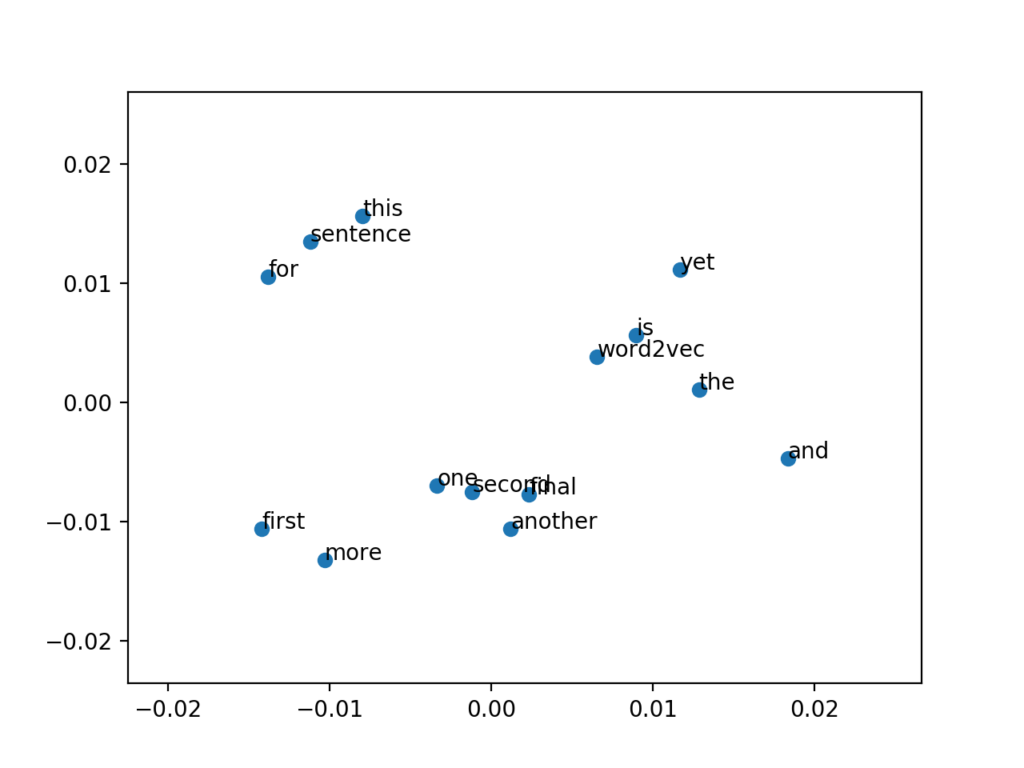
\includegraphics[width=0.45\linewidth,keepaspectratio]{gensim1}
\end{center}

Note: It is hard to pull much meaning out of the graph given such a tiny corpus was used to fit the model.

\end{frame}


%%%%%%%%%%%%%%%%%%%%%%%%%%%%%%%%%%%%%%%%%%%%%%%%%%%%%%%%%%%%%%%%%%%%%%%%%%%%%%%%%%
\begin{frame}[fragile]\frametitle{Using Google's pre-trained word vectors}
\begin{itemize}
\item Use google's pre-trained model. It contains word vectors for a vocabulary of 3 million words trained on around 100 billion words from the google news dataset.
\item Beware it is a 1.5 GB download.
\end{itemize}
\begin{lstlisting}
from gensim.models import Word2Vec

model = Word2Vec.load_word2vec_format('GoogleNews-vectors-negative300.bin', binary=True, norm_only=True)
# getting word vectors of a word
dog = model['dog']
#performing king queen magic
print(model.most_similar(positive=['woman', 'king'], negative=['man']))
#printing similarity index
print(model.similarity('woman', 'man'))
\end{lstlisting}
\end{frame}


%%%%%%%%%%%%%%%%%%%%%%%%%%%%%%%%%%%%%%%%%%%%%%%%%%%%%%%%%%%%%%%%%%%%%%%%%%%%%%%%%%
\begin{frame}[fragile]\frametitle{Using Stanford’s GloVe word vectors}
\begin{itemize}
\item Stanford researchers also have their own word embedding algorithm like word2vec called Global Vectors for Word Representation, or GloVe for short.
\item You can download the GloVe pre-trained word vectors and load them easily with gensim.
\end{itemize}
\begin{lstlisting}
from gensim.scripts.glove2word2vec import glove2word2vec
glove_input_file = 'glove.6B.100d.txt'
word2vec_output_file = 'glove.6B.100d.txt.word2vec'
glove2word2vec(glove_input_file, word2vec_output_file)
\end{lstlisting}
You now have a copy of the GloVe model in word2vec format with the filename glove.6B.100d.txt.word2vec.
\end{frame}

%%%%%%%%%%%%%%%%%%%%%%%%%%%%%%%%%%%%%%%%%%%%%%%%%%%%%%%%%%%%%%%%%%%%%%%%%%%%%%%%%%
\begin{frame}[fragile]\frametitle{Using Stanford’s GloVe word vectors}
\begin{lstlisting}
from gensim.models import Word2Vec

model = Word2Vec.load_word2vec_format('glove.6B.100d.txt.word2vec',binary=False)
# getting word vectors of a word
dog = model['dog']
#performing king queen magic
print(model.most_similar(positive=['woman', 'king'], negative=['man']))
#printing similarity index
print(model.similarity('woman', 'man'))
\end{lstlisting}
\end{frame}


%%%%%%%%%%%%%%%%%%%%%%%%%%%%%%%%%%%%%%%%%%%%%%%%%%%%%%%%%%%%%%%%%%%%%%%%%%%%%%%%%%
\begin{frame}[fragile]\frametitle{}

\begin{center}
{\Large Doc2Vec}
\end{center}

{\tiny (Ref: DOC2VEC gensim tutorial - Deepak Mishra)}
\end{frame}

%%%%%%%%%%%%%%%%%%%%%%%%%%%%%%%%%%%%%%%%%%%%%%%%%%%%%%%%%%%%%%%%%%%%%%%%%%%%%%%%%%
\begin{frame}[fragile]\frametitle{Import libraries and Load the Data and tag it}
\begin{lstlisting}
from gensim.models.doc2vec import Doc2Vec, TaggedDocument
from nltk.tokenize import word_tokenize

data = ["I love machine learning. Its awesome.",
        "I love coding in python",
        "I love building chatbots",
        "they chat amazingly well"]
		
tagged_data = [TaggedDocument(words=word_tokenize(_d.lower()), tags=[str(i)]) for i, _d in enumerate(data)]		
\end{lstlisting}

Here we have a list of four sentences as training data and each sentence acts as a document.

\end{frame}


%%%%%%%%%%%%%%%%%%%%%%%%%%%%%%%%%%%%%%%%%%%%%%%%%%%%%%%%%%%%%%%%%%%%%%%%%%%%%%%%%%
\begin{frame}[fragile]\frametitle{Training}

\begin{lstlisting}
max_epochs = 100
vec_size = 20
alpha = 0.025

model = Doc2Vec(size=vec_size,
                alpha=alpha, 
                min_alpha=0.00025,
                min_count=1,
                dm =1)
  
model.build_vocab(tagged_data)

for epoch in range(max_epochs):
    print('iteration {0}'.format(epoch))
    model.train(tagged_data,
                total_examples=model.corpus_count,
                epochs=model.iter)
    # decrease the learning rate
    model.alpha -= 0.0002
    # fix the learning rate, no decay
    model.min_alpha = model.alpha

model.save("d2v.model")
print("Model Saved")
\end{lstlisting}
\end{frame}

%%%%%%%%%%%%%%%%%%%%%%%%%%%%%%%%%%%%%%%%%%%%%%%%%%%%%%%%%%%%%%%%%%%%%%%%%%%%%%%%%%
\begin{frame}[fragile]\frametitle{Hyperparameter: ``dm''}
\begin{itemize}
\item dm defines the training algorithm. If dm=1 means ‘distributed memory’ (PV-DM) and dm =0 means ‘distributed bag of words’ (PV-DBOW). 
\item Distributed Memory model preserves the word order in a document whereas Distributed Bag of words just uses the bag of words approach, which doesn’t preserve any word order.
\end{itemize}

\end{frame}

%%%%%%%%%%%%%%%%%%%%%%%%%%%%%%%%%%%%%%%%%%%%%%%%%%%%%%%%%%%%%%%%%%%%%%%%%%%%%%%%%%
\begin{frame}[fragile]\frametitle{Use the model}
\begin{lstlisting}
from gensim.models.doc2vec import Doc2Vec

model= Doc2Vec.load("d2v.model")
#to find the vector of a document which is not in training data
test_data = word_tokenize("I love chatbots".lower())
v1 = model.infer_vector(test_data)
print("V1_infer", v1)

# to find most similar doc using tags
similar_doc = model.docvecs.most_similar('1')
print(similar_doc)


# to find vector of doc in training data using tags or in other words, printing the vector of document at index 1 in training data
print(model.docvecs['1'])
\end{lstlisting}

\end{frame}


%%%%%%%%%%%%%%%%%%%%%%%%%%%%%%%%%%%%%%%%%%%%%%%%%%%%%%%%%%%%%%%%%%%%%%%%%%%%%%%%%%
\begin{frame}[fragile]\frametitle{}

\begin{center}
{\Large Comparison of Vectorization}
\end{center}

{\tiny (Ref: Gensim Tutorial-2: Word2Vec and Doc2Vec)}
\end{frame}

%%%%%%%%%%%%%%%%%%%%%%%%%%%%%%%%%%%%%%%%%%%%%%%%%%%%%%%%%%%%%%%%%%%%%%%%%%%%%%%%%%
\begin{frame}[fragile]\frametitle{Vectorization (recap)}
\begin{itemize}
\item What do vectors do? 
\item They represent our text in mathematical forms so we can use them in computation.
\item To find similarity
\item Their constituents can be used as features for Machine Learning Algorithms
\item Here we will demonstrate various vectorization methods built on same dataset, so one can compare.
\end{itemize}
\end{frame}


%%%%%%%%%%%%%%%%%%%%%%%%%%%%%%%%%%%%%%%%%%%%%%%%%%%%%%%%%%%%%%%%%%%%%%%%%%%%%%%%%%
\begin{frame}[fragile]\frametitle{Creating a Toy Corpus}
\begin{lstlisting}
import pandas as pd
import numpy as np

CORPUS = [
'the green car is fast',
'The blue car has low mileage',
'Your car has high mileage',
'I buy green shirt because it fits my blue eyes'
]

new_doc = ['I want to buy a car']
\end{lstlisting}
\end{frame}


%%%%%%%%%%%%%%%%%%%%%%%%%%%%%%%%%%%%%%%%%%%%%%%%%%%%%%%%%%%%%%%%%%%%%%%%%%%%%%%%%%
\begin{frame}[fragile]\frametitle{Bag Of Words}
\begin{lstlisting}
from sklearn.feature_extraction.text import CountVectorizer
def bow_generator(corpus, ngram_range=(1,2)):
    vectorizer = CountVectorizer(min_df=1, ngram_range=ngram_range)
    features = vectorizer.fit_transform(corpus)
    return vectorizer, features


# build bow vectorizer and get features
bow_vectorizer, bow_features = bow_generator(CORPUS)
features = bow_features.todense()
print (features)
***
[[0 0 0 0 0 0 0 1 0 1 0 1 0 0 1 1 0 0 0 0 0 0 1 1 0 0 0 0 0 0 0 0 0 1 0 1
  0 0]
 [0 0 1 1 0 0 0 1 1 0 0 0 0 0 0 0 0 1 0 1 0 0 0 0 0 0 1 1 1 0 0 0 0 1 1 0
  0 0]
 [0 0 0 0 0 0 0 1 1 0 0 0 0 0 0 0 0 1 1 0 1 1 0 0 0 0 0 0 1 0 0 0 0 0 0 0
  1 1]
 [1 1 1 0 1 1 1 0 0 0 1 0 1 1 1 0 1 0 0 0 0 0 0 0 1 1 0 0 0 1 1 1 1 0 0 0
  0 0]]
\end{lstlisting}
Each document has been converted to vectors. Each row represents one document from our corpus. Note that we used bigrams in our model.
\end{frame}


%%%%%%%%%%%%%%%%%%%%%%%%%%%%%%%%%%%%%%%%%%%%%%%%%%%%%%%%%%%%%%%%%%%%%%%%%%%%%%%%%%
\begin{frame}[fragile]\frametitle{Bigrams}
\begin{lstlisting}
# print the feature names
feature_names = bow_vectorizer.get_feature_names()
print (feature_names)
***
['because', 'because it', 'blue', 'blue car', 'blue eyes', 'buy', 'buy green', 'car', 'car has', 'car is',
 'eyes', 'fast', 'fits', 'fits my', 'green', 'green car', 'green shirt', 'has', 'has high', 'has low', 
'high', 'high mileage', 'is', 'is fast', 'it', 'it fits', 'low', 'low mileage', 'mileage', 'my', 'my blue',
 'shirt', 'shirt because', 'the', 'the blue', 'the green', 'your', 'your car']
\end{lstlisting}

\end{frame}

%%%%%%%%%%%%%%%%%%%%%%%%%%%%%%%%%%%%%%%%%%%%%%%%%%%%%%%%%%%%%%%%%%%%%%%%%%%%%%%%%%
\begin{frame}[fragile]\frametitle{Dataframe}
\begin{lstlisting}
# extract features from new document using built vectorizer
new_doc_features = bow_vectorizer.transform(new_doc)
new_doc_features = new_doc_features.todense()
print(new_doc_features)
***
[[0 0 0 0 0 1 0 1 0 0 0 0 0 0 0 0 0 0 0 0 0 0 0 0 0 0 0 0 0 0 0 0 0 0 0 0 0 0]]

df_train = pd.DataFrame(data=features, columns=feature_names)
\end{lstlisting}
Data frame should look like below:

\begin{center}
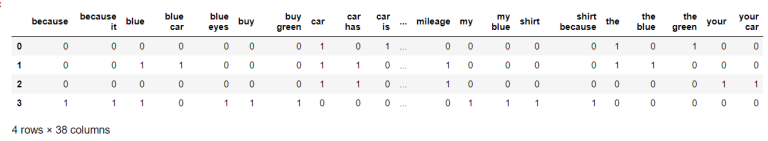
\includegraphics[width=\linewidth,keepaspectratio]{emb1}
\end{center}
\end{frame}

%%%%%%%%%%%%%%%%%%%%%%%%%%%%%%%%%%%%%%%%%%%%%%%%%%%%%%%%%%%%%%%%%%%%%%%%%%%%%%%%%%
\begin{frame}[fragile]\frametitle{Dataframe}
\begin{center}
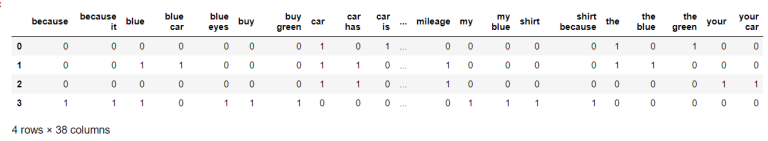
\includegraphics[width=\linewidth,keepaspectratio]{emb1}
\end{center}

\begin{itemize}
\item Columns show the words in our dictionary, and the value is the frequency of that word in the document. 
\item Note that for the new document–new\_doc, there is no feature for many words because the feature-extraction process, model, and vocabulary are always based on the training data. 
\item It will not be influenced by newer documents. 
\item The features in this model are based on the vector space of the training corpus.
\end{itemize}
\end{frame}


%%%%%%%%%%%%%%%%%%%%%%%%%%%%%%%%%%%%%%%%%%%%%%%%%%%%%%%%%%%%%%%%%%%%%%%%%%%%%%%%%%
\begin{frame}[fragile]\frametitle{Tf-IDF (recap)}
\begin{itemize}
\item TF-IDF is the product of two metrics: term frequency (TF) and inverse-document frequency (IDF). \item The term TF is what we had computed in the bag of words model (the raw frequencies of terms). Inverse document frequency, IDF, is computed by dividing the total number of documents in our corpus by the document frequency for each term and then applying logarithmic scaling on the result. 
\item  The IDF is a measure of how much information the term provides through checking whether it is common or rare across all documents.
\end{itemize}
\end{frame}

%%%%%%%%%%%%%%%%%%%%%%%%%%%%%%%%%%%%%%%%%%%%%%%%%%%%%%%%%%%%%%%%%%%%%%%%%%%%%%%%%%
\begin{frame}[fragile]\frametitle{Tf-IDF}
\begin{lstlisting}
from sklearn.feature_extraction.text import TfidfTransformer
transformer = TfidfTransformer(norm='l2',smooth_idf=True, use_idf=True) #smoothing gives sme weights to terms with zero idf not to ignore them.
tfidf_matrix = transformer.fit_transform(bow_features)
features = np.round(tfidf_matrix.todense(), 2)

df_tfidf = pd.DataFrame(data=features, columns=feature_names)
df_tfidf
\end{lstlisting}
\begin{center}
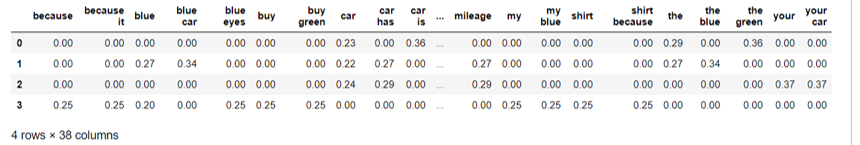
\includegraphics[width=\linewidth,keepaspectratio]{emb2}
\end{center}
\end{frame}

%%%%%%%%%%%%%%%%%%%%%%%%%%%%%%%%%%%%%%%%%%%%%%%%%%%%%%%%%%%%%%%%%%%%%%%%%%%%%%%%%%
\begin{frame}[fragile]\frametitle{Tf-IDF}
\begin{lstlisting}
# tfidf features for new_doc
tfidf_matrix = transformer.fit_transform(new_doc_features)
features_new = np.round(tfidf_matrix.todense(), 2)

df_tfidf_new = pd.DataFrame(data=features_new, columns=feature_names)
df_tfidf_new
\end{lstlisting}
\begin{center}
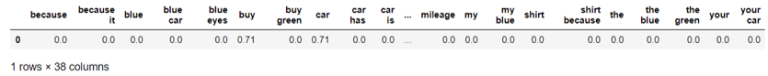
\includegraphics[width=\linewidth,keepaspectratio]{emb3}
\end{center}
\end{frame}


%%%%%%%%%%%%%%%%%%%%%%%%%%%%%%%%%%%%%%%%%%%%%%%%%%%%%%%%%%%%%%%%%%%%%%%%%%%%%%%%%%
\begin{frame}[fragile]\frametitle{Word2Vec}
\begin{lstlisting}
import gensim # commonly used for semantic analysis, topic modeling and similarity analysis.
import nltk
# tokenize corpora
TOKENIZED_CORPUS = [nltk.word_tokenize(sentence) for sentence in CORPUS]
tokenized_new_doc = [nltk.word_tokenize(sentence) for sentence in new_doc]
# build the word2vec model on our training corpus
model = gensim.models.Word2Vec(TOKENIZED_CORPUS, size=5, window=2, min_count=1)
print (model.wv['green'])
print (model.wv['blue'])
***
[-0.0911594   0.0799796   0.06533758 -0.07235344 -0.04641258]
[-0.02380046 -0.09778572  0.08745811  0.00992521  0.04947698]
\end{lstlisting}
\end{frame}

%%%%%%%%%%%%%%%%%%%%%%%%%%%%%%%%%%%%%%%%%%%%%%%%%%%%%%%%%%%%%%%%%%%%%%%%%%%%%%%%%%
\begin{frame}[fragile]\frametitle{}

\begin{center}
{\Large Building Doc2Vec for Movie Reviews corpus}
\end{center}

{\tiny (Ref: How to Develop a Word Embedding Model for Predicting Movie Review Sentiment - Jason Brownlee)}
\end{frame}

%%%%%%%%%%%%%%%%%%%%%%%%%%%%%%%%%%%%%%%%%%%%%%%%%%%%%%%%%%%%%%%%%%%%%%%%%%%%%%%%%%
\begin{frame}[fragile]\frametitle{Movie Review Dataset}
\begin{itemize}
\item Movie reviews retrieved from the imdb.com website in the early 2000s by Bo Pang and Lillian Lee.
\item The dataset is comprised of 1,000 positive and 1,000 negative movie reviews drawn from an archive of the rec.arts.movies.reviews newsgroup hosted at imdb.com. The authors refer to this dataset as the “polarity dataset.”
\item The data has been cleaned up somewhat, for example:
\begin{itemize}
\item The dataset is comprised of only English reviews.
\item All text has been converted to lowercase.
\item There is white space around punctuation like periods, commas, and brackets.
\item Text has been split into one sentence per line.
\end{itemize}
\end{itemize}
\end{frame}

%%%%%%%%%%%%%%%%%%%%%%%%%%%%%%%%%%%%%%%%%%%%%%%%%%%%%%%%%%%%%%%%%%%%%%%%%%%%%%%%%%
\begin{frame}[fragile]\frametitle{Movie Review Dataset}
\begin{itemize}
\item Source: http://www.cs.cornell.edu/people/pabo/movie-review-data/review\_polarity.tar.gz (3MB)
\item After unzipping the file, you will have a directory called “txt\_sentoken” with two sub-directories containing the text “neg” and “pos” for negative and positive reviews. 
\item Reviews are stored one per file with a naming convention cv000 to cv999 for each neg and pos.
\end{itemize}
\end{frame}

%%%%%%%%%%%%%%%%%%%%%%%%%%%%%%%%%%%%%%%%%%%%%%%%%%%%%%%%%%%%%%%%%%%%%%%%%%%%%%%%%%
\begin{frame}[fragile]\frametitle{Loading and Cleaning Reviews}
The text data is already pretty clean; but still \ldots
\begin{itemize}
\item Split tokens on white space.
\item Remove all punctuation from words.
\item Remove all words that are not purely comprised of alphabetical characters.
\item Remove all words that are known stop words.
\item Remove all words that have a length $<= 1$ character.
\end{itemize}
\end{frame}

%%%%%%%%%%%%%%%%%%%%%%%%%%%%%%%%%%%%%%%%%%%%%%%%%%%%%%%%%%%%%%%%%%%%%%%%%%%%%%%%%%
\begin{frame}[fragile]\frametitle{Sample File Loading and Cleaning}
\begin{lstlisting}
from nltk.corpus import stopwords
import string
 
# load doc into memory
def load_doc(filename):
	# open the file as read only
	file = open(filename, 'r')
	# read all text
	text = file.read()
	# close the file
	file.close()
	return text
\end{lstlisting}
\end{frame}

%%%%%%%%%%%%%%%%%%%%%%%%%%%%%%%%%%%%%%%%%%%%%%%%%%%%%%%%%%%%%%%%%%%%%%%%%%%%%%%%%%
\begin{frame}[fragile]\frametitle{Sample File Loading and Cleaning}
\begin{lstlisting}
# turn a doc into clean tokens
def clean_doc(doc):
	# split into tokens by white space
	tokens = doc.split()
	# remove punctuation from each token
	table = str.maketrans('', '', string.punctuation)
	tokens = [w.translate(table) for w in tokens]
	# remove remaining tokens that are not alphabetic
	tokens = [word for word in tokens if word.isalpha()]
	# filter out stop words
	stop_words = set(stopwords.words('english'))
	tokens = [w for w in tokens if not w in stop_words]
	# filter out short tokens
	tokens = [word for word in tokens if len(word) > 1]
	return tokens
\end{lstlisting}
\end{frame}

%%%%%%%%%%%%%%%%%%%%%%%%%%%%%%%%%%%%%%%%%%%%%%%%%%%%%%%%%%%%%%%%%%%%%%%%%%%%%%%%%%
\begin{frame}[fragile]\frametitle{Sample File Loading and Cleaning}
\begin{lstlisting}
# load the document
filename = 'data/txt_sentoken/pos/cv000_29590.txt'
text = load_doc(filename)
tokens = clean_doc(text)
print(tokens)

...
'creepy', 'place', 'even', 'acting', 'hell', 'solid', 'dreamy', 'depp', 'turning', 'typically', 'strong', 'performance', 'deftly', 'handling', 'british', 'accent', 'ians', 'holm', 'joe', 'goulds', 'secret', 'richardson', 'dalmatians', 'log', 'great', 'supporting', 'roles', 'big', 'surprise', 'graham', 'cringed', 'first', 'time', 'opened', 'mouth', 'imagining', 'attempt', 'irish', 'accent', 'actually', 'wasnt', 'half', 'bad', 'film', 'however', 'good', 'strong', 'violencegore', 'sexuality', 'language', 'drug', 'content']
\end{lstlisting}
\end{frame}


%%%%%%%%%%%%%%%%%%%%%%%%%%%%%%%%%%%%%%%%%%%%%%%%%%%%%%%%%%%%%%%%%%%%%%%%%%%%%%%%%%
\begin{frame}[fragile]\frametitle{Define a Vocabulary}
\begin{itemize}
\item Vocabulary means all the words in the corpus, like a mini dictionary. 
\item We can develop a vocabulary as a Counter, which is a dictionary mapping of words and their counts that allow us to easily update and query.
\item Each document can be added to the counter (a new function called add\_doc\_to\_vocab()) and we can step over all of the reviews in the negative directory and then the positive directory (a new function called process\_docs()).
\end{itemize}
\end{frame}

%%%%%%%%%%%%%%%%%%%%%%%%%%%%%%%%%%%%%%%%%%%%%%%%%%%%%%%%%%%%%%%%%%%%%%%%%%%%%%%%%%
\begin{frame}[fragile]\frametitle{Define a Vocabulary}
\begin{lstlisting}
from string import punctuation
from os import listdir
from collections import Counter

def add_doc_to_vocab(filename, vocab):
	doc = load_doc(filename)
	tokens = clean_doc(doc)
	# update counts
	vocab.update(tokens)

# load all docs in a directory
def process_docs(directory, vocab, is_trian):
	# walk through all files in the folder
	for filename in listdir(directory):
		# skip any reviews in the test set
		if is_trian and filename.startswith('cv9'):
			continue
		if not is_trian and not filename.startswith('cv9'):
			continue
		path = directory + '/' + filename
		add_doc_to_vocab(path, vocab)
\end{lstlisting}
\end{frame}

%%%%%%%%%%%%%%%%%%%%%%%%%%%%%%%%%%%%%%%%%%%%%%%%%%%%%%%%%%%%%%%%%%%%%%%%%%%%%%%%%%
\begin{frame}[fragile]\frametitle{Define a Vocabulary}
\begin{lstlisting}
from string import punctuation
from os import listdir
from collections import Counter

# define vocab
vocab = Counter()
# add all docs to vocab
process_docs('txt_sentoken/neg', vocab, True)
process_docs('txt_sentoken/pos', vocab, True)
# print the size of the vocab
print(len(vocab))
44276
\end{lstlisting}
Running the example shows that we have a vocabulary of 44,276 words.
\end{frame}

%%%%%%%%%%%%%%%%%%%%%%%%%%%%%%%%%%%%%%%%%%%%%%%%%%%%%%%%%%%%%%%%%%%%%%%%%%%%%%%%%%
\begin{frame}[fragile]\frametitle{See the Vocabulary}
We also can see a sample of the top 50 most used words in the movie reviews.
Note, that this vocabulary was constructed based on only those reviews in the training dataset.

\begin{lstlisting}
# print the top words in the vocab
print(vocab.most_common(50))


[('film', 7983), ('one', 4946), ('movie', 4826), ('like', 3201), ('even', 2262), ('good', 2080), ('time', 2041), ('story', 1907), ('films', 1873), ('would', 1844), ('much', 1824), ('also', 1757), ('characters', 1735), ('get', 1724), ('character', 1703), ('two', 1643), ('first', 1588), ('see', 1557), ('way', 1515), ('well', 1511), ('make', 1418), ('really', 1407), ('little', 1351), ('life', 1334), ('plot', 1288), ('people', 1269), ('could', 1248), ('bad', 1248), ('scene', 1241), ('movies', 1238), ('never', 1201), ('best', 1179), ('new', 1140), ('scenes', 1135), ('man', 1131), ('many', 1130), ('doesnt', 1118), ('know', 1092), ('dont', 1086), ('hes', 1024), ('great', 1014), ('another', 992), ('action', 985), ('love', 977), ('us', 967), ('go', 952), ('director', 948), ('end', 946), ('something', 945), ('still', 936)]
\end{lstlisting}
Running the example shows that we have a vocabulary of 44,276 words.
\end{frame}

%%%%%%%%%%%%%%%%%%%%%%%%%%%%%%%%%%%%%%%%%%%%%%%%%%%%%%%%%%%%%%%%%%%%%%%%%%%%%%%%%%
\begin{frame}[fragile]\frametitle{Prune the Vocabulary}
We can step through the vocabulary and remove all words that have a low occurrence, such as only being used once or twice in all reviews.

\begin{lstlisting}
# keep tokens with a min occurrence
min_occurane = 2
tokens = [k for k,c in vocab.items() if c >= min_occurane]
print(len(tokens))

25767
\end{lstlisting}
Running the above example with this addition shows that the vocabulary size drops by a little more than half its size from 44,276 to 25,767 words.
\end{frame}

%%%%%%%%%%%%%%%%%%%%%%%%%%%%%%%%%%%%%%%%%%%%%%%%%%%%%%%%%%%%%%%%%%%%%%%%%%%%%%%%%%
\begin{frame}[fragile]\frametitle{Save the Vocabulary}
Finally, the vocabulary can be saved to a new file called vocab.txt that we can later load and use to filter movie reviews prior to encoding them for modeling. We define a new function called save\_list() that saves the vocabulary to file, with one word per file.

\begin{lstlisting}
# save list to file
def save_list(lines, filename):
	# convert lines to a single blob of text
	data = '\n'.join(lines)
	# open file
	file = open(filename, 'w')
	# write text
	file.write(data)
	# close file
	file.close()

# save tokens to a vocabulary file
save_list(tokens, 'vocab.txt')
\end{lstlisting}
Running the min occurrence filter on the vocabulary and saving it to file, you should now have a new file called vocab.txt with only the words we are interested in.
\end{frame}

%%%%%%%%%%%%%%%%%%%%%%%%%%%%%%%%%%%%%%%%%%%%%%%%%%%%%%%%%%%%%%%%%%%%%%%%%%%%%%%%%%
\begin{frame}[fragile]\frametitle{Train word2vec Embedding}
Loading the vocabulary

\begin{lstlisting}
# load doc into memory
def load_doc(filename):
	# open the file as read only
	file = open(filename, 'r')
	# read all text
	text = file.read()
	# close the file
	file.close()
	return text

# load the vocabulary
vocab_filename = 'vocab.txt'
vocab = load_doc(vocab_filename)
vocab = vocab.split()
vocab = set(vocab)
\end{lstlisting}

\end{frame}

%%%%%%%%%%%%%%%%%%%%%%%%%%%%%%%%%%%%%%%%%%%%%%%%%%%%%%%%%%%%%%%%%%%%%%%%%%%%%%%%%%
\begin{frame}[fragile]\frametitle{Train word2vec Embedding}
Go to each document, clean it and keep only words from the VOCAB.

\begin{lstlisting}
# turn a doc into clean tokens
def doc_to_clean_lines(doc, vocab):
	clean_lines = list()
	lines = doc.splitlines()
	for line in lines:
		# split into tokens by white space
		tokens = line.split()
		# remove punctuation from each token
		table = str.maketrans('', '', punctuation)
		tokens = [w.translate(table) for w in tokens]
		# filter out tokens not in vocab
		tokens = [w for w in tokens if w in vocab]
		clean_lines.append(tokens)
	return clean_lines
\end{lstlisting}

\end{frame}

%%%%%%%%%%%%%%%%%%%%%%%%%%%%%%%%%%%%%%%%%%%%%%%%%%%%%%%%%%%%%%%%%%%%%%%%%%%%%%%%%%
\begin{frame}[fragile]\frametitle{Train word2vec Embedding}
Next, we adapt the process\_docs() function to load and clean all of the documents in a folder and return a list of all document lines
\begin{lstlisting}
# load all docs in a directory
def process_docs(directory, vocab, is_trian):
	lines = list()
	# walk through all files in the folder
	for filename in listdir(directory):
		# skip any reviews in the test set
		if is_trian and filename.startswith('cv9'):
			continue
		if not is_trian and not filename.startswith('cv9'):
			continue
		# create the full path of the file to open
		path = directory + '/' + filename
		# load and clean the doc
		doc = load_doc(path)
		doc_lines = doc_to_clean_lines(doc, vocab)
		# add lines to list
		lines += doc_lines
	return lines
\end{lstlisting}

\end{frame}

%%%%%%%%%%%%%%%%%%%%%%%%%%%%%%%%%%%%%%%%%%%%%%%%%%%%%%%%%%%%%%%%%%%%%%%%%%%%%%%%%%
\begin{frame}[fragile]\frametitle{Train word2vec Embedding}
We can then load all of the training data and convert it into a long list of ‘sentences’ (lists of tokens) ready for fitting the word2vec model.
\begin{lstlisting}
# load training data
positive_lines = process_docs('txt_sentoken/pos', vocab, True)
negative_lines = process_docs('txt_sentoken/neg', vocab, True)
sentences = negative_docs + positive_docs
print('Total training sentences: %d' % len(sentences))
\end{lstlisting}

\end{frame}

%%%%%%%%%%%%%%%%%%%%%%%%%%%%%%%%%%%%%%%%%%%%%%%%%%%%%%%%%%%%%%%%%%%%%%%%%%%%%%%%%%
\begin{frame}[fragile]\frametitle{Train word2vec Embedding}
\begin{itemize}
\item The model is fit when constructing the class. 
\item  We pass in the list of clean sentences from the training data, then specify the size of the embedding vector space (we use 100 again), the number of neighboring words to look at when learning how to embed each word in the training sentences (we use 5 neighbors), the number of threads to use when fitting the model (we use 8, but change this if you have more or less CPU cores), and the minimum occurrence count for words to consider in the vocabulary (we set this to 1 as we have already prepared the vocabulary).
\end{itemize}

\begin{lstlisting}
# train word2vec model
model = Word2Vec(sentences, size=100, window=5, workers=8, min_count=1)
# summarize vocabulary size in model
words = list(model.wv.vocab)
print('Vocabulary size: %d' % len(words))
\end{lstlisting}

\end{frame}

%%%%%%%%%%%%%%%%%%%%%%%%%%%%%%%%%%%%%%%%%%%%%%%%%%%%%%%%%%%%%%%%%%%%%%%%%%%%%%%%%%
\begin{frame}[fragile]\frametitle{Train word2vec Embedding}
Finally, we save the learned embedding vectors to file using the save\_word2vec\_format() on the model’s ‘wv‘ (word vector) attribute. The embedding is saved in ASCII format with one word and vector per line.
\begin{lstlisting}
# save model in ASCII (word2vec) format
filename = 'data/embedding_word2vec.txt'
model.wv.save_word2vec_format(filename, binary=False)

\end{lstlisting}
Running the example loads 58,109 sentences from the training data and creates an embedding for a vocabulary of 25,767 words.

You should now have a file ’embedding\_word2vec.txt’ with the learned vectors in your data directory.
\end{frame}

